\documentclass[../main.tex]{subfiles}




\begin{document}

\chapter{}
\label{cha:cha_3}


\section{}
The M-file can be written as
\bigbreak
\begin{lstlisting}[numbers=none]
function sincomp(x,n)
i = 1;
tru = sin(x);
ser = 0;
fprintf('\n');
fprintf('order true value approximation error\n');
while (1)
 if i > n, break, end
 ser = ser + (-1)^(i - 1) * x^(2*i-1) / factorial(2*i-1);
 er = (tru - ser) / tru * 100;
 fprintf('%3d %14.10f %14.10f %12.8f\n',i,tru,ser,er);
 i = i + 1;
end
\end{lstlisting}
\bigbreak
This function can be used to evaluate the test case, 
\bigbreak
\begin{lstlisting}[numbers=none]
>> sincomp(1.5,8)

order  true value    approximation    error
 1		 0.9974949866 	1.5000000000 -50.37669564
 2 		 0.9974949866 	0.9375000000	 6.01456523
 3		 0.9974949866 	1.0007812500 	-0.32945162
 4 		 0.9974949866 	0.9973911830 	 0.01040643
 5		 0.9974949866 	0.9974971226 	-0.00021414
 6 		 0.9974949866	  0.9974949557	 0.00000310
 7  	 0.9974949866	  0.9974949869	-0.00000003
 8 		 0.9974949866	  0.9974949866	 0.00000000
\end{lstlisting}
\bigbreak
\section{}
The M-file can be written as
\bigbreak
\begin{lstlisting}[numbers=none]
function futureworth(P, i, n)
nn = 0:n;
F = P*(1+i).^nn;
y = [nn;F];
fprintf('\n year future worth\n');
fprintf('%5d %14.2f\n',y);
\end{lstlisting}
\bigbreak
This function can be used to evaluate the test case, 
\bigbreak
\begin{lstlisting}[numbers=none]
>> futureworth(100000,0.08,8)

 year future worth
   0 		100000.00
   1 		108000.00
   2 		116640.00
   3 		125971.20
   4 		136048.90
   5 		146932.81
   6 		158687.43
   7 		171382.43
   8 		185093.02 
\end{lstlisting}
\bigbreak\bigbreak
\section{}
The M-file can be written as 
\bigbreak

\begin{lstlisting}[numbers=none]
function annualpayment(P, i, n)
nn = 1:n;
A = P*i*(1+i).^nn./((1+i).^nn-1);
y = [nn;A];
fprintf('\n year annualpayment\n');
fprintf('%5d %14.2f\n',y);
\end{lstlisting}
\bigbreak
This function can be used to evaluate the test case, 
\bigbreak
\begin{lstlisting}[numbers=none]
>> annualpayment(35000,.076,5)

 year 	annualpayment
   1 			 37660.00
   2 			 19519.34
   3 			 13483.26
   4 			 10473.30
   5 			 8673.76 
\end{lstlisting}
\bigbreak
\section{}
The M-file can be written as
\bigbreak
\begin{lstlisting}[numbers=none]
function Tavg = avgtemp(Tmean, Tpeak, tstart, tend)
omega = 2*pi/365;
t = tstart:tend;
Te = Tmean + (Tpeak-Tmean)*cos(omega*(t-205));
Tavg = mean(Te);
\end{lstlisting}
\bigbreak
This function can be used to evaluate the test cases,
\bigbreak
\begin{lstlisting}[numbers=none]
>> avgtemp(5.2,22.1,0,59)

ans =
 -10.8418

>> avgtemp(23.1,33.6,180,242)

ans =
 33.0398 
\end{lstlisting}
\bigbreak
\section{}
The M-file can be written as
\bigbreak
\begin{lstlisting}[numbers=none]
function vol = tankvol(R, d)
if d < R
 vol = pi * d ^ 3 / 3;
elseif d <= 3 * R
 v1 = pi * R ^ 3 / 3;
 v2 = pi * R ^ 2 * (d - R);
 vol = v1 + v2;
else
 error('overtop')
end 
\end{lstlisting}\bigbreak
This function can be used to evaluate the test cases, 
\bigbreak
\begin{lstlisting}[numbers=none]
>> tankvol(1,0.5)
ans =
 0.1309

>> tankvol(1,1.2)
ans =
 1.6755

>> tankvol(1,3.0)
ans =
 7.3304

>> tankvol(1,3.1)
??? Error using ==> tankvol
overtop
\end{lstlisting}
\bigbreak
\section{}
The M-file can be written as
\bigbreak
\begin{lstlisting}[numbers=none]
function [r, th] = polar(x, y)
r = sqrt(x .^ 2 + y .^ 2);
if x < 0
  if y > 0
    th = atan(y / x) + pi;
  elseif y < 0
    th = atan(y / x) - pi;
  else
    th = pi;
  end
else
  if y > 0
    th = pi / 2;
  elseif y < 0
    th = -pi / 2;
  else
    th = 0;
  end
end
th = th * 180 / pi;
\end{lstlisting}
\bigbreak
This function can be used to evaluate the test cases. For example, for the first case,
\bigbreak
\begin{lstlisting}[numbers=none]
>> [r,th]=polar(1,1)

r =
 1.4142

th =
 90
\end{lstlisting}
\bigbreak
The remaining cases are 
\bigbreak
\begin{tabular}{cccc}
\Xhline{1.5pt}
$x$ & $y$ & $r$ & $\theta$ \\
\hline
1 & 1 & $1.4142$ & 90 \\
1 & $-1$ & $1.4142$ & $-90$ \\
1 & 0 & $1.0000$ & 0 \\
$-1$ & 1 & $1.4142$ & 135 \\
$-1$ & $-1$ & $1.4142$ & $-135$ \\
$-1$ & 0 & $1.0000$ & 180 \\
0 & 1 & $1.0000$ & 90 \\
0 & $-1$ & $1.0000$ & $-90$ \\
0 & 0 & $0.0000$ & 0 \\
\Xhline{1.5pt}
\end{tabular}
\bigbreak
\section{}
The M-file can be written as
\bigbreak
\begin{lstlisting}[numbers=none]
function polar2(x, y)
r = sqrt(x .^ 2 + y .^ 2);
n = length(x);
for i = 1:n
  if x(i) < 0
    if y(i) > 0
      th(i) = atan(y(i) / x(i)) + pi;
    elseif y(i) < 0
      th(i) = atan(y(i) / x(i)) - pi;
    else
      th(i) = pi;
    end
  else
    if y(i) > 0
      th(i) = pi / 2;
    elseif y(i) < 0
      th(i) = -pi / 2;
    else
      th(i) = 0;
    end
  end
  th(i) = th(i) * 180 / pi;
end
ou = [x;y;r;th];
fprintf('\n x y radius angle\n');
fprintf('%8.2f %8.2f %10.4f %10.4f\n',ou);
\end{lstlisting}
\bigbreak
This function can be used to evaluate the test cases and display the results in tabular form
\bigbreak
\begin{lstlisting}[numbers=none]
>> polar2(x,y)

  x 			y 		radius 		 angle
 1.00 	 1.00 	1.4142 	  90.0000
 1.00 	-1.00 	1.4142 	 -90.0000
 1.00  	 0.00 	1.0000 	   0.0000
-1.00	   1.00	 	1.4142   135.0000
-1.00	  -1.00	  1.4142  -135.0000
-1.00    0.00 	1.0000 	 180.0000
 0.00 	 1.00 	1.0000	  90.0000
 0.00 	-1.00 	1.0000	 -90.0000
 0.00	   0.00 	0.0000 	   0.0000 
\end{lstlisting}
\bigbreak
\section{}
The M-file can be written as
\bigbreak

\begin{lstlisting}[numbers=none]
function grade = lettergrade(score)
if score >= 90
  grade = 'A';
elseif score >= 80
  grade = 'B';
elseif score >= 70
  grade = 'C';
elseif score >= 60
  grade = 'D';
else
  grade = 'F';
end 
\end{lstlisting}
\bigbreak
This function can be tested with a few cases,
\bigbreak
\begin{lstlisting}[numbers=none]
>> lettergrade(95)
ans =
A

>> lettergrade(45)
ans =
F

>> lettergrade(80)
ans =
B 
\end{lstlisting}
\bigbreak
\section{}
The M-file can be written as
\bigbreak
\begin{lstlisting}[numbers=none]
function Manning(A)
A(:,5)= sqrt(A(:,2))./A(:,1).*(A(:,3).*A(:,4)./(A(:,3)+2*A(:,4))).^(2/3);
fprintf('\n    n         S          B          H          U\n');
fprintf('%8.3f %8.4f %10.2f %10.2f %10.4f\n',A');
\end{lstlisting}
\bigbreak
This function can be run to create the table,
\bigbreak
\begin{lstlisting}[numbers=none]
>> Manning(A)

	  n         S         B         H          U             
	 0.035 	 0.0001 	  10.00 		 2.00		  0.3624
 	 0.020 	 0.0002 	   8.00 		 1.00		  0.6094
	 0.015   0.0010 	  20.00 		 1.50 	  2.5167
	 0.030   0.0007 	  24.00	 	   3.00 		1.5809
	 0.022   0.0003 	  15.00	 	   2.50		  1.1971
\end{lstlisting}
\bigbreak
\section{}
The M-file can be written as
\bigbreak
\begin{lstlisting}[numbers=none]
function beam(x)
xx = linspace(0,x
n=length(xx);
for i=1:n
  uy(i) = -5/6.*(sing(xx(i),0,4)-sing(xx(i),5,4));
  uy(i) = uy(i) + 15/6.*sing(xx(i),8,3) + 75*sing(xx(i),7,2);
  uy(i) = uy(i) + 57/6.*xx(i)^3 - 238.25.*xx(i);
end
plot(xx,uy)

function s = sing(xxx,a,n)
if xxx > a
  s = (xxx - a).^n;
else
  s=0;
end 
\end{lstlisting}
\bigbreak
This function can be run to create the plot,
\bigbreak
\begin{lstlisting}[numbers=none]
>> beam(10)
\end{lstlisting}
\bigbreak
\begin{figure}[H]
		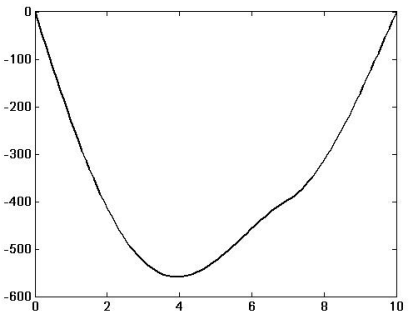
\includegraphics[width=0.5\linewidth]{fig_3_1}
		\label{fig:fig_3_1}
	\end{figure}
\bigbreak
\section{}
The M-file can be written as
\bigbreak
\begin{lstlisting}[numbers=none]
function cylinder(r, L)
h = linspace(0,2*r);
V = (r^2*acos((r-h)./r)-(r-h).*sqrt(2*r*h-h.^2))*L;
plot(h, V)
\end{lstlisting}
\bigbreak
This function can be run to the plot,
\bigbreak
\begin{lstlisting}[numbers=none]
>> cylinder(2,5)
\end{lstlisting}
\bigbreak
\begin{figure}[H]
		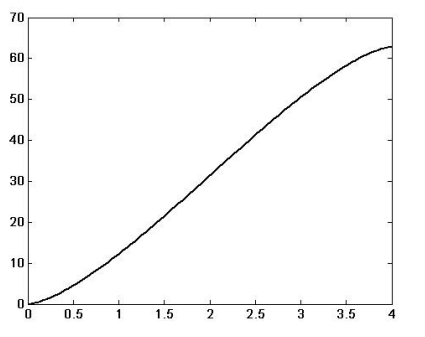
\includegraphics[width=0.5\linewidth]{fig_3_2}
		\label{fig:fig_3_2}
	\end{figure}
\end{document}

